\documentclass[ignorenonframetext,]{beamer}
\setbeamertemplate{caption}[numbered]
\setbeamertemplate{caption label separator}{: }
\setbeamercolor{caption name}{fg=normal text.fg}
\beamertemplatenavigationsymbolsempty
\usepackage{lmodern}
\usepackage{amssymb,amsmath}
\usepackage{ifxetex,ifluatex}
\usepackage{fixltx2e} % provides \textsubscript
\ifnum 0\ifxetex 1\fi\ifluatex 1\fi=0 % if pdftex
  \usepackage[T1]{fontenc}
  \usepackage[utf8]{inputenc}
\else % if luatex or xelatex
  \ifxetex
    \usepackage{mathspec}
  \else
    \usepackage{fontspec}
  \fi
  \defaultfontfeatures{Ligatures=TeX,Scale=MatchLowercase}
\fi
% use upquote if available, for straight quotes in verbatim environments
\IfFileExists{upquote.sty}{\usepackage{upquote}}{}
% use microtype if available
\IfFileExists{microtype.sty}{%
\usepackage{microtype}
\UseMicrotypeSet[protrusion]{basicmath} % disable protrusion for tt fonts
}{}
\newif\ifbibliography
\hypersetup{
            pdftitle={GDR EcoStats - CiSStats 2019},
            pdfauthor={Simon},
            pdfborder={0 0 0},
            breaklinks=true}
\urlstyle{same}  % don't use monospace font for urls
\usepackage{graphicx,grffile}
\makeatletter
\def\maxwidth{\ifdim\Gin@nat@width>\linewidth\linewidth\else\Gin@nat@width\fi}
\def\maxheight{\ifdim\Gin@nat@height>\textheight0.8\textheight\else\Gin@nat@height\fi}
\makeatother
% Scale images if necessary, so that they will not overflow the page
% margins by default, and it is still possible to overwrite the defaults
% using explicit options in \includegraphics[width, height, ...]{}
\setkeys{Gin}{width=\maxwidth,height=\maxheight,keepaspectratio}

% Prevent slide breaks in the middle of a paragraph:
\widowpenalties 1 10000
\raggedbottom

\AtBeginPart{
  \let\insertpartnumber\relax
  \let\partname\relax
  \frame{\partpage}
}
\AtBeginSection{
  \ifbibliography
  \else
    \let\insertsectionnumber\relax
    \let\sectionname\relax
    \frame{\sectionpage}
  \fi
}
\AtBeginSubsection{
  \let\insertsubsectionnumber\relax
  \let\subsectionname\relax
  \frame{\subsectionpage}
}

\setlength{\parindent}{0pt}
\setlength{\parskip}{6pt plus 2pt minus 1pt}
\setlength{\emergencystretch}{3em}  % prevent overfull lines
\providecommand{\tightlist}{%
  \setlength{\itemsep}{0pt}\setlength{\parskip}{0pt}}
\setcounter{secnumdepth}{0}

\title{GDR EcoStats - CiSStats 2019}
\author{Simon}
\date{}

\begin{document}
\frame{\titlepage}

\begin{frame}{Galaxy Bricks : une plateforme d'analyse de données
collaborative}

Simon Bénateau, Sébastien Turpin, Yvan Le Bras

Les sciences participatives ont pour objectif historique le recueil de
données. La plateforme ``Galaxy-Bricks'' contribue à l'élargissement du
champ d'action de celles-ci en offrant la possibilité aux participants
de prendre part à l'analyse de données. La possibilité de comprendre
comment les chercheurs analysent les données et de participer à ces
analyses devrait susciter de nouveaux modes de collaboration entre la
recherche et les citoyens. Les outils de partage de résultats, d'outils,
de workflow et de rapport que propose ``Galaxy-E'' couplés au cadre de
formation proposés par le réseau ``Galaxy training material'' permettent
d'atteindre ces objectifs.

\end{frame}

\begin{frame}{Galaxy Ecology : Une plateforme d'analyse de données
accessible.}

Simon Bénateau, Benjamin Yguel, Alan Amossé, Sébastien Turpin, Yvan Le
Bras

\end{frame}

\begin{frame}{Vigie nature}

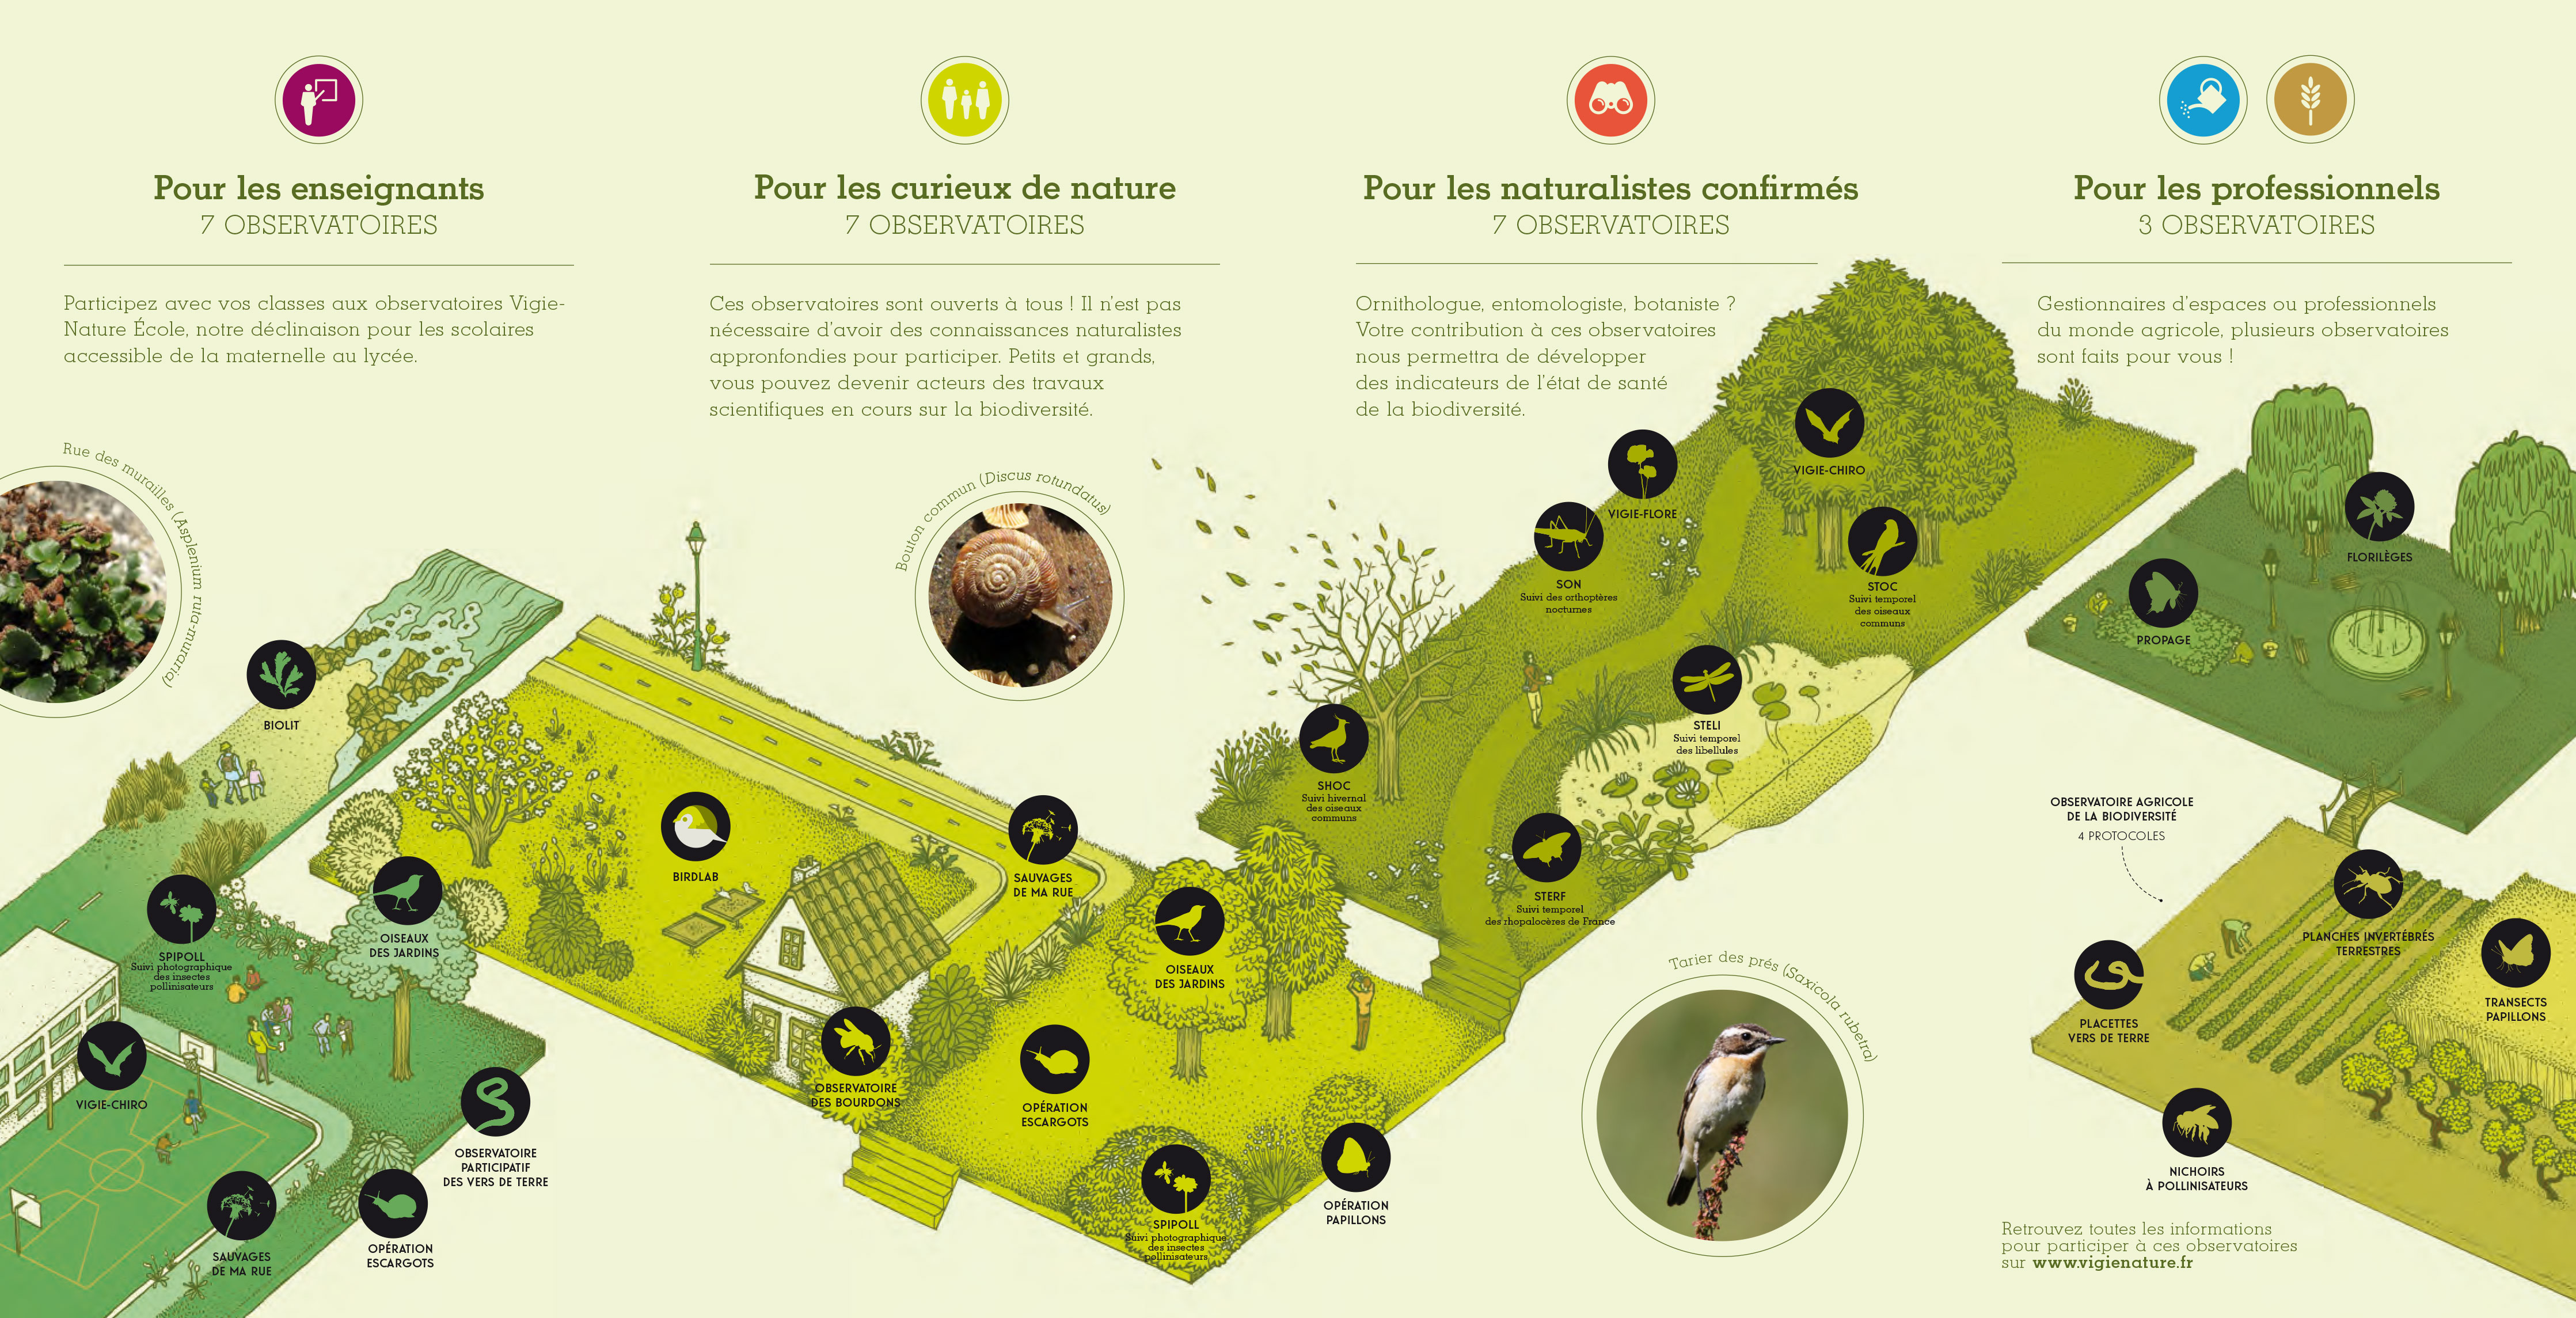
\includegraphics{figures/observatoires_vigienature.jpg}

\end{frame}

\begin{frame}{Organisation du réseau d'acteur}

\begin{center}  
\includegraphic[figures/Vigie-Nature-Network.jpg]
\end{center}

\end{frame}

\begin{frame}{La place de l'analyse de données et de la production
d'indicateurs}

\end{frame}

\begin{frame}{Demandes de la communautés et freins à l'implémentation}

\begin{itemize}
\tightlist
\item
  Dépendances (versions des packages)
\item
  Lignes de commande (utilisation de R)
\end{itemize}

\end{frame}

\begin{frame}{Perspective}

FAIR

\begin{itemize}
\tightlist
\item
  Tutoriels
\end{itemize}

L'analyse des données issues des obervatoires de scicences
participatives nécessite l'emploi d'outils statistiques pointus qui
requièrent des compétences en programmation. Ces dernières peuvent
représenter un obstacle à l'apprentissage ou à l'utilisation d'outils
par certains acteurs de la communautés des sciences participatives. La
plateforme galaxy-E permet de développer des outils avec une interface
graphique, gérant les dépendances et la reproductibilité des analyses.
Elle facilite l'accès à ces outils pour les acteurs des sciences
participatives qui analysent les données et produisent des indicateurs.

Nous vous présenterons les derniers développement des outils de la
plateforme et sur les projets

\end{frame}

\end{document}
